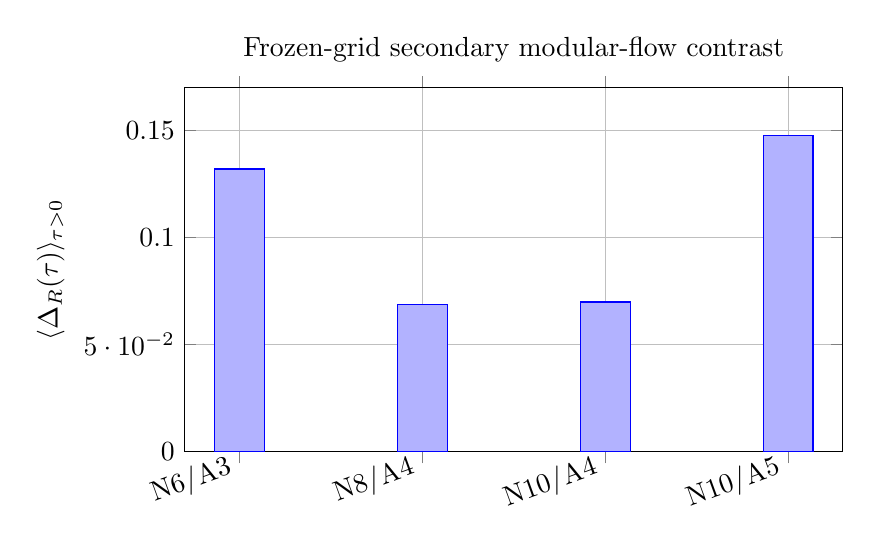
\begin{tikzpicture}
\begin{axis}[
  width=0.82\textwidth,height=6.2cm,
  ybar,bar width=18pt,
  ymin=0,ymax=0.17,
  ylabel={$\langle\Delta_R(\tau)\rangle_{\tau>0}$},
  symbolic x coords={N6/A3,N8/A4,N10/A4,N10/A5},
  xtick=data,
  x tick label style={rotate=20,anchor=east},
  title={Frozen-grid secondary modular-flow contrast},
  grid=major
]
\addplot coordinates {(N6/A3,0.1320520591) (N8/A4,0.0687091263) (N10/A4,0.0699112761) (N10/A5,0.1479409231)};
\end{axis}
\end{tikzpicture}
